\documentclass{article}
\title{This is my first document}
\author{Vaclav Klecanda}
\date{31.1.2009}
\begin{document}

\section*{submission}
Study available literature and technical documentation about programming on IBM Cell BE architecture. As well as interfaces, development environments and tools for creating programs for CellBE and its particular implementation Play Station 3, IBM system simulator, Cell Blade. Find out its potential and abilities for parallel processing. Learn about design patterns.

Try some algorithm (registration, segmentation) aimed to medical data processing (CT, MR, X-ray images) where huge data sizes are processed and where results has to be get relativelly fast because diagnosis are made for lasg number of patients. It suitable to do comparation study between common PC architecture and CellBE aimed to speed, precision, code complexity and ways of algorithms design itselfs.

\chapter{Introduction}

Since first processors of x86 platform were released big race for who introduce processor with operating on higher frequency started.
This was conditioned to research new production technologies that allow to integrated more transistors onto smaller area.
In the process manufacturers started to realize that it is impossible to continue this frequency race forever.
This results integration of more computing units into single processor.
This first among common desktop processors was Intel's Pentium\textsuperscript{\textregistered} with hyper threading.
This processors was able to execute two threads at a time.
Since then quick boom of multi-core integration started even among other biggest processor manufacturers.
Integration of more execution cores allows less power consumption.
This factor is nowadays especially important due to processor integration into laptops and even due to environmental issues.
That's why current efforts of processor manufacturers is to gain the best performance to power consumption ratio.

Cores that are integrated into the current processors are general purpose.
This means they have pipeline for instruction execution with several stages.
Instruction can be with several states within such pipeline, e.g. fetched, awaiting operands, ready, executed.
Instruction flows among the stages not in the order they are within the program.
Order is decided by the processor based on variety factors and predictions.
One of the pipeline stages is branch prediction unit that has to predict the most probable flow of the executed program.
When this prediction is false whole pipeline has to be discarded and execution of the right branch of program has to be started.
Processors suffer heavily from mispredictions because they lead into big holes in which the processor pipeline stalls or is being reset.

Another general purpose processor suffering is from cache misses.
This occurs when requested data are not within processor cache and have to be load from memory.

Altough many of improvements were implemented into the general purpose processors they still suffer from the described problems.
This is one of the reasons why collaboration of three big companies IBM, Sony, and Toshiba started development of Cell B.E. processor.
Processor that is multi-core, has good performance to power consumption ratio and is able to overcome the problems that the general purpose processors suffer.
Because it allow the programmer to somewhat manage processor cache and branch prediction unit.

\chapter{Cell B.E. platform}

This chapter will introduce Cell Broadband Engine processor (Cell B.E.) and the whole platform and its specific details.
Particular Cell B.E. processor will be described and illustrated.

\section{About the processor}

Cell B.E. processor is representative of a new generation of IBM's Cell B.E. platform family.
Cell B.E. is an asymmetric, high-performance multi-core processor that combines eight synergistic processing elements (SPEs) and a Power Processing Element (PPE), which is a general-purpose IBM Power PC\textsuperscript{\textregistered} core.
Next part is a central memory element.
PPE can operate with the central memory directly while SPE indirectly, see below.
In Cell B.E. are several kinds of memories.
All the elements are connected through high speed bus (EIB - Element Interconnect Bus).
Whole layout is on figure \ref{fg:processorLayout}.

\begin{figure}
    \centering
    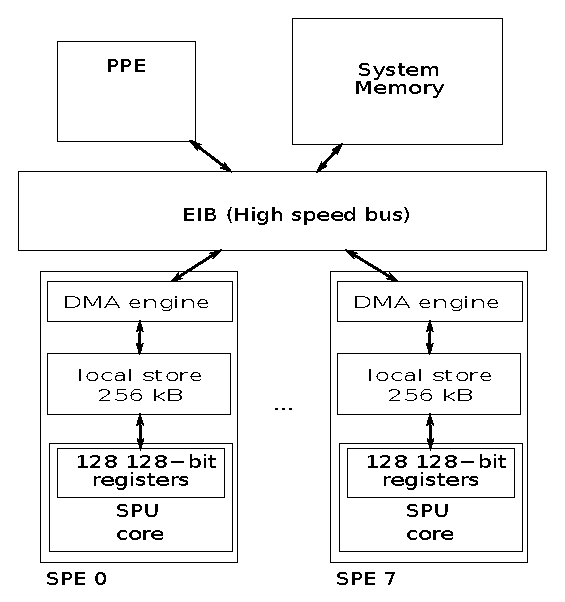
\includegraphics[width=0.7\textwidth]{data/cellLayout}
    \caption[Cell B.E. processor layout]{One PPE unit along with eight SPE stream processor units and system memory connected together with high speed EIB bus}
    \label{fg:processorLayout}
\end{figure}

Cell B.E. achieves a significant performance per Watt and performance per chip area advantage over conventional high-performance processors.
Is significantly more flexible and programmable than single-function and other optimized processors such as graphics processors, or conventional digital signal processors.
While a conventional microprocessor may deliver about 20+GFlops of single-precision (32b) floating-point performance, Cell delivers 200+ GFlops (in ideal conditions) at comparable power.

A number of signal processing and media applications have been implemented on Cell with excellent results.
Advanced visualization such as ray-casting, ray-tracing, and volume rendering.
Or streaming applications such as media encoders, decoders or encryption and decryption standards have also been demonstrated to perform about an order of magnitude better than conventional PC.


\subsection{PPE - Power Processing Element}
PPE is derived from IBM Power PC\textsuperscript{\textregistered} core. Has 512kB L2 cache on die.
It supports the Power Architecture ISA, inherits the memory translation, protection, and SMP coherence model of mainstream 64-bit Power processors.
CBEA also supports virtualization (logical partitioning), large pages, and other recent innovations in the Power architecture.
Programming for the PPE is the same as for conventional processors due to direct access to central memory.

\subsection{SPE - Synergistic Processing Element}

\par
SPE is an autonomous processor (sometimes called accelerator) targeted for computational intensive applications.
Each SPE has a SIMD core (SPU), a high-speed private local store memory and a direct memory access (DMA) engine.
The SPU unit has 128 128-bit wide unified general purpose (in contrast from traditional RISCs where registers are divided according data types) registers to store all types of data.
It supports a SIMD-RISC instruction set.
It can execute two instruction at one clock tick in some conditions (dual-issue).
Vectorized operations in various data types configurations can be performed with these registers.
E.g. two double-precision floats or eight 32bit integers can be processed at single clock tick.

\par
Unlike conventional microprocessors, SPE does not have a hardware cache.
Its function supply the small on-chip local store memory under programmer's control.
This allow code optimizations that can reduce cache misses.
The local store is separated from the main memory (on which the PPE operates), so SPE has its own address space.
Therefore any synchronization with other cores is not necessary.
The local store is attached to a larger (central) shared memory through DMA engine that manages transferring data from central memory to local store and vice versa as well as between two local stores.
We say that data is "DMAed" from source to destination.
DMA commands can be issued in many ways.
Synchronous, asynchronous, in scatter-gather manner through DMA lists.
Therefore, this Cell B.E. can be viewed as a distributed memory multiprocessor.
This memory management is another big part of programming for Cell B.E..

\par
Programming for SPE has some differences over programming for conventional processor.
Programmer have always to count with the fact that have only 256kB for the program and data.

\par
This processor is embeded in Sony Playstation 3 game console as well as IBM Blade servers where two or more such processors (as building blocks) connected by high speed bus creates powerfull and modular machine.
We have Play Station 3 (PS3) machine available for this work.
\chapter {\mbox{Cell/B.E.} programming}
\par
\mbox{Cell/B.E.} platform development tools will be described in this chapter.
Our experience with the tools will be mentioned as well.
Then particular SDK content and tools will be listed.
Parallel systems and models will be mentioned later on as well as the relationship to the \mbox{Cell/B.E.} development along with a few design patterns.
At the end core configurations and their advantages and disadvantages will be listed finishing with few practical approaches to the \mbox{Cell/B.E.} porting process.

\section{\mbox{Cell/B.E.} platform development}
\par
IBM delivers a SDK for the \mbox{Cell/B.E.} application development.
It is made for a Linux platform, in the concrete for the Fedora or the Red Hat distribution.
It comes in two flavours.
The first is the official non free SDK which has all the features needed for the \mbox{Cell/B.E.} development even for hybrid systems.
The purchaser has also a support team ready to help.
The next is a free one that is open to wide public and everybody can download it and start developing.
The free one does not have full support for hybrid systems nor for development in other languages than C/C++.
We have used the free one since we have developed only in C/C++ and for a clean \mbox{Cell/B.E.} processor.

\par
Because the SDK is for Linux operation system its user has to have already a deeper knowledge about this system.
There are a few bugs and parts that are not fully finished (see Appendix \ref{toolsSetup}) and without the deeper system knowledge is practically impossible to react on an unexpected behaviour during installation or development phase.

\par
We have begun with SDK version 3.0 and Fedora version 8 which were the current versions of needed tools.
We have faced a number of obstacles and before we were able to overcome them a new version of SDK (3.1) appeared.
Because we wanted to use and describe the latest tools we had to begin from scratch because the new version brought new obstacles as well.

\par
The new version was declared to be compatible with a new version of Fedora, 9 - Sulphur, that had been released at almost the same time as the new SDK version.
The previous version of SDK (3.0) was for Fedora 7 Werewolf.
We have tried all possible combinations of Fedora distributions and SDK packages to find out if they are compatible with each other.
The only result from that testings was finding out that they are not mutually compatible.
We have spent plenty of days on this discovery.
The SDK is a huge package of software dependent on lots of third party libraries and solutions.
They are treated differently within particular distributions and sometimes even versions of the same distribution.
The resulting advise is to avoid combination of system versions nor SDK versions nor particular libraries that the SDK components are dependent on.
The repository versions of the third party software should be used.

\par
Although there are too much of troubles when different version are combined, a few efforts to get the SDK run on another distributions than Fedora were made.
But we think the time spent on this goal is not worth the result.

\par
Finally we installed Fedora 9 Sulphur and SDK 3.1.
Although this combination is declared by IBM as tested we have run into few bugs and errors.
The process of installation is described in the Appendix \ref{toolsSetup}.

\section {SDK content}

The \mbox{Cell/B.E.} SDK is divided into variety of components.
Each component is contained in one or more rpm package for easy installation purposes.
Here is a list of important available components:
\begin{enumerate}
  \item {Tool chain}
  \par
  Is a set of tools such as compilers, linkers etc. necessary for actual code generation.
There are two tool chains.
One is for PPU and the other for SPU.

  \item {Libraries}
  \par
  IBM provides several useful libraries for mathematical purposes e.g. linear algebra, FFT, Monte Carlo with the SDK.
Another libraries set is for cryptography or SPE run-time management.
Code of these libraries is debugged, highly optimized for running on SPEs and SIMDized.
It is highly advisible to use the libraries i.e. adapt a code for using the libraries instead of programming own solution.\\

  \item {Full system simulator}
  \par
  Program that can simulate the \mbox{Cell/B.E.} processor on other hardware platforms.
It is used mostly in profiling stage because simulator can simulate actual computation of a code in cycle precision.
It can be of course used when programmer has an actual \mbox{Cell/B.E.} hardware available, but the simulation is incredibly slow.

  \item {IDE}
  \par
  IDE is in fact version 3.2 of Eclipse with integration of debugging, profiling, \mbox{Cell/B.E.} machine management and other features that makes development for the \mbox{Cell/B.E.} easier and more comfortable.
\end{enumerate}


\section{Parallel systems \& \mbox{Cell/B.E.}}

Parallelism depends on type of system where the program will be run.
There are two basic kind of parallel systems:
\begin{enumerate}
\item {shared-memory system}
\par
Is a multi-processor system with one shared memory which all processor can see.
Processors has to synchronize access to the memory otherwise race conditions will rise.

\item {distributed-memory system}
\par
Is system where each processor has its own private memory.
There is no need for any synchronization.
\end{enumerate}

In context of parallel systems \mbox{Cell/B.E.} is a kind of hybrid system.
The SPEs matches a distributed-memory system due to private local stores while the PPE is a shared-memory system.
The \mbox{Cell/B.E.} is sometimes called heterogeneous multi-core processor with distributed memory.
Because \mbox{Cell/B.E.} processors can be composed into bigger units such as IBM blade server with two \mbox{Cell/B.E.} chips they can be viewed as either \mbox{16 + 2} cores in SMP mode or two non-uniform memory access machines connected together.
Programmer has then to decide which view of the \mbox{Cell/B.E.} processor is better for the solved problem.

\par
Because of separation of address spaces programming of the SPE is very similar to client/server application design.
Roles depends on how the work is started.
In case the PPU initiates the transfers, the PPU is a client and the SPE is a server because the SPE receive data for computation and offer a service for the PPE.
Another possibility is that the SPE grabs the data from the central memory.
In this case the SPE is a client of central memory.
This scenario is preferred because the PPE is only one and would not be able to manage all the SPUs.

\section{\mbox{Cell/B.E.} programming models}

\par
Implementation of parallel algorithms rely on a parallel programming model.
It is a set of software technologies such as programming languages extension, special compilers, libraries through that actual parallelism is achieved.
The programming model is programmer's view to the hardware.
Choosing a programming model or mixture of models that will best fit for the solved problem is another decision that programmer has to make.

\par
For the \mbox{Cell/B.E.} there is variety of parallel programming models.
THe models differ in view of the hardware from each other and thus how many actions are performed implicitly by the model.
The actions can be e.g. task distribution management, data distribution management or synchronization.
The most abstract ones can perform many actions implicitly.
Their advantage is ease of implementation but at cost no performance tuning ability.
Differently act the most concrete models that see the \mbox{Cell/B.E.} processor with all the low level details.
Their advantage is performance tuning ability in all application parts but at cost of more development.

\par
There are several models that are targeted only for the \mbox{Cell/B.E.} platform and are contained in the SDK.
While there are other models such as MPI, OpenMP that can be used as well but they would expose only the PPE.
These will not be further described.

List of the programming models (frameworks) follows in order from the most concrete to the most abstract:
\begin{enumerate}
\item {libspe2}
\par
This library provides the most low level functionality.
It offers SPE context creating, running, scheduling or deleting.
DMA primitives for data transfer, mailboxes, signal, events, and synchronization functions for PPE to SPE and SPE to SPE dialogues are also provided by this library.
More information can be found in \cite{performanceToolRef} within "SPE Runtime Management Library" document.

\item {Data Communication and Synchronization - DaCS}
\par
Defines a program entity for the PPE or the SPE.
It is a HE (Host Element program) for the PPE and an AE (Accelerator Element program) for the SPE.
It provides variety of services for that programs.
The services are e.g. resource and process management where an HE manipulates its AEs or group management, for defining groups in which synchronization events like barriers can happen or message passing by using send and receive primitives.
More information can be found in \cite{performanceToolRef} within "DACS Programmer's Guide and API Reference" document.\\\\

\item {Accelerated Library Framework - ALF}
\par
The ALF defines an ALF-task as another entity that perform computationally intensive parts of a program.
The idea is to have a program split into multiple independent pieces which are called work blocks.
They are described by a computational kernel, the input and the output data.
Programming with the ALF is divided into two sides.
The host and the accelerator one.
On the accelerator side the programmer has only to code the computational kernel, unwrap the input data, and pack the output data when the kernel finishes.
The ALF offers clear separation between the host and the accelerator sides of program parts.
It provides following services: work blocks queue management, load balancing between accelerators, transparent DMA transfers etc.
More information can be found in \cite{performanceToolRef} within "ALF Programmer's Guide and API Reference" document.

\end{enumerate}

Choosing a framework is important decision of writing \mbox{Cell/B.E.} application.
It should be considered enough.

\subsection {\mbox{Cell/B.E.} parallelism levels}

The \mbox{Cell/B.E.} processor offers four levels of parallel processing.
That is because it is composed of heterogeneous elements, the SPE and the PPE and the possibility of composition into a more complex systems.
The levels are:
\begin{enumerate}
\item Server level
\par
Parallelism on this level means task distribution among multiple servers like within a server farm.
This is possible in a hybrid environment at the cluster level using MPI or some other grid computing middle-ware.

\item \mbox{Cell/B.E.} chips level
\par
On this level tasks can be divided among multiple \mbox{Cell/B.E.} processors.
This is possible if there are more such processors in single machine.
It is e.g. IBM Blade server with two \mbox{Cell/B.E.} chips.
ALF or DaCS for hybrid can be used for task distribution.

\item SPE level
\par
This parallelism level allows to distribute tasks among particular SPEs.
Libspe, ALF, DaCS can be used to perform the distribution.

\item SIMD instruction level
\par
This level can increase the speed the most.
Parallelism is achieved on instruction level that means more data are processed at a time by single instruction.
Language intrinsics are used for this purpose.
This will be explained later in part devoted to "SIMDation".
\end{enumerate}

\subsection{Computation configurations}

\par
Because of the \mbox{Cell/B.E.}'s heterogeneous nature there are few computation configurations that can be used.
Each of them differs in usage of SPEs:
\begin{enumerate}
\item Streaming configuration
\par
All SPEs serves as a stream processor (see figure \ref{fg:streamingModel}).
They run exactly the same code expecting the same type of data and producing also the same of data type.
This configuration is well suited for streaming application for example filters where there is still the same type of data on input.

\begin{figure}
    \centering
    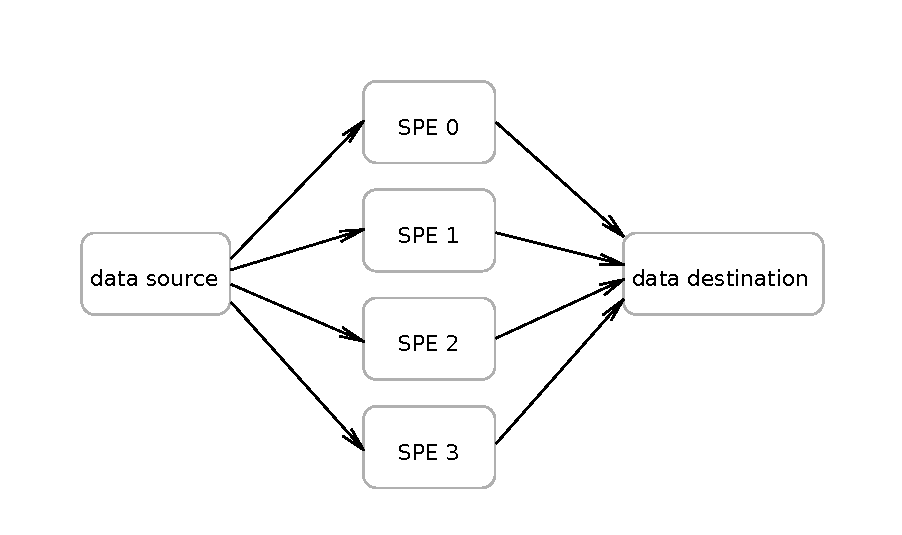
\includegraphics[width=0.9\textwidth]{data/streamingModel}
    \caption[Streaming SPE configuration]{All SPE run the same code creating farm of processor that process same type of data.}
    \label{fg:streamingModel}
\end{figure}

\item Pipeline configuration
\par
The SPEs are stages of a pipeline (see figure \ref{fg:pipelineModel}).
Data are passed through one SPE to another.
This configuration makes use of the fact that transfer among SPEs is faster than the transfer between SPE and PPE.

\begin{figure}
    \centering
    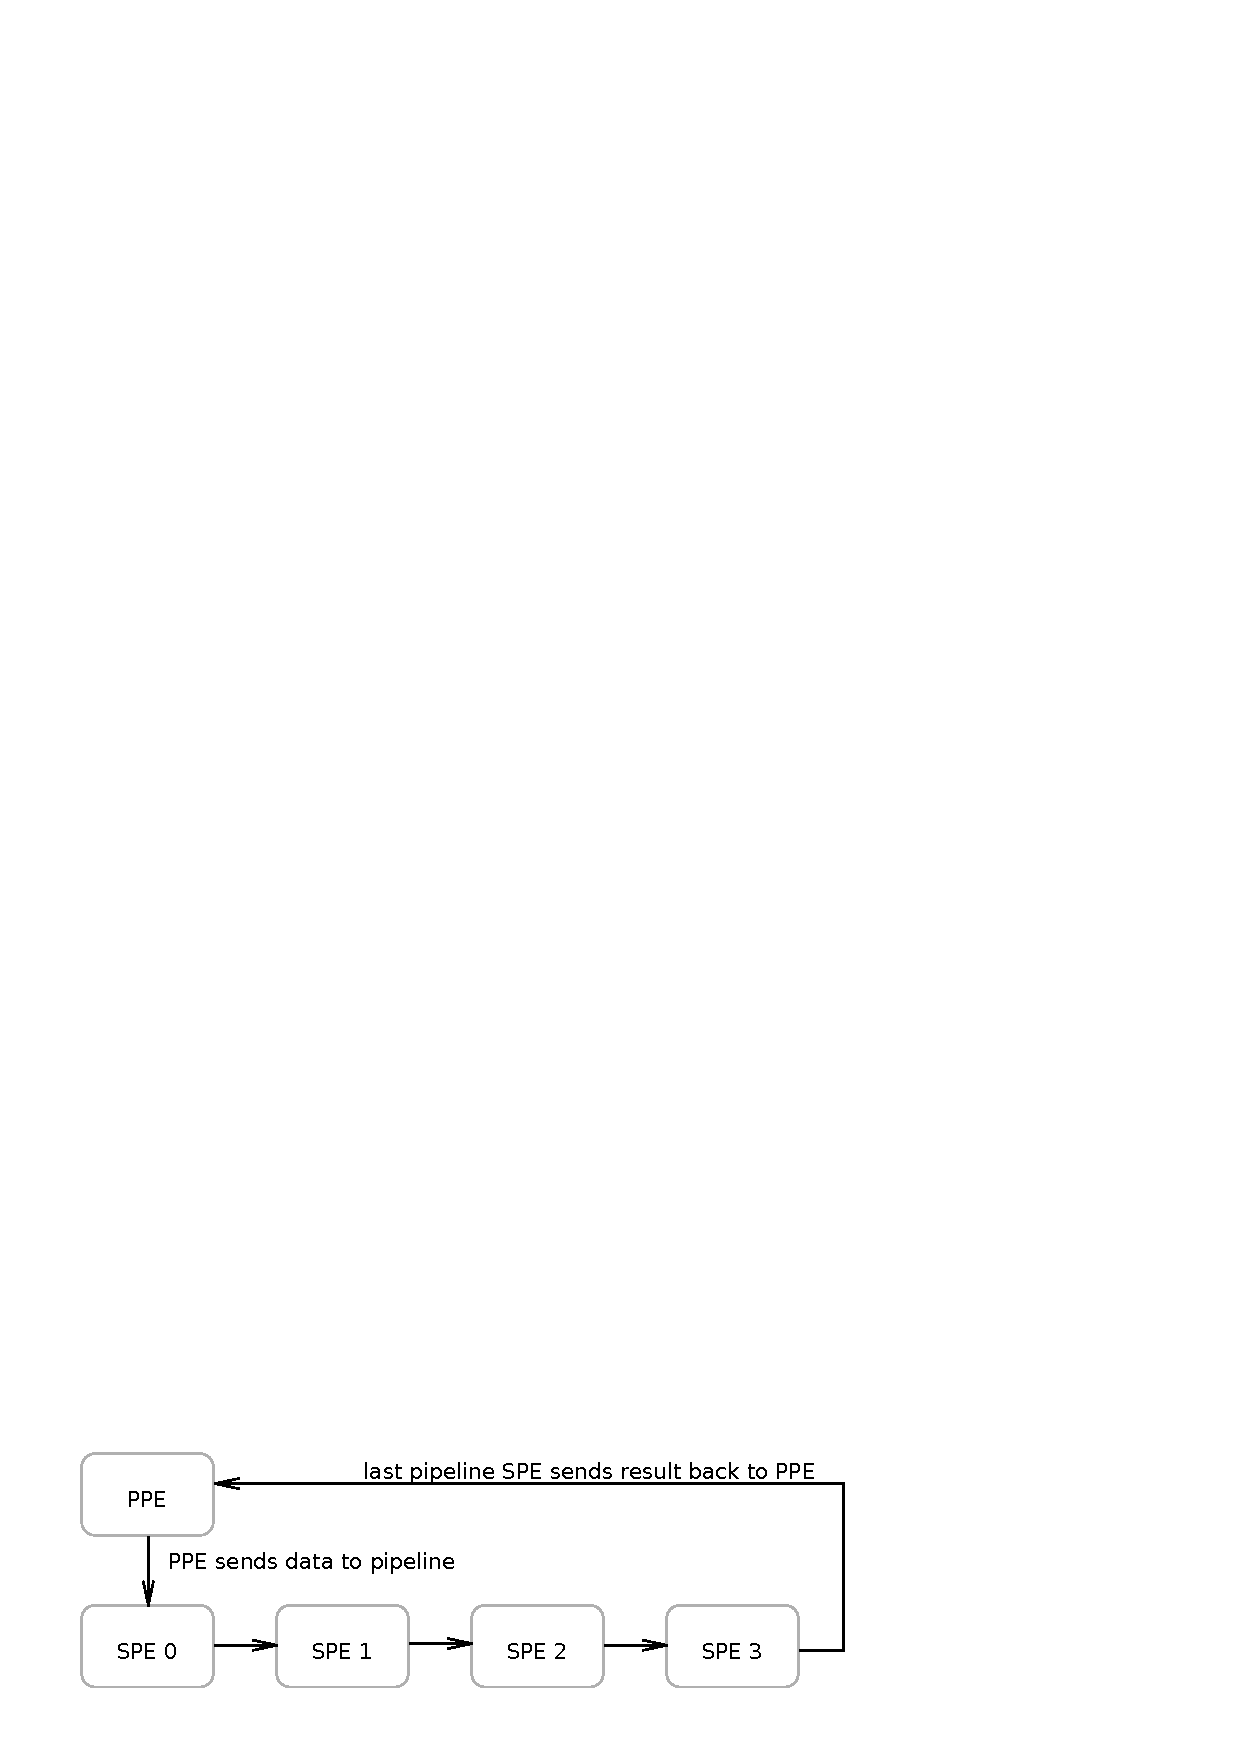
\includegraphics[width=0.9\textwidth]{data/pipelineModel}
    \caption[Pipeline SPE configuration]{SPE creates a pipeline. Each SPE represent one stage of that pipeline. Data are transferred only via SPE to SPE DMA transfers benefiting the speed of bus.}
    \label{fg:pipelineModel}
\end{figure}

\item PPE centric
\par
This configuration is common approach to use the \mbox{Cell/B.E.}
A program runs on the PPE (see figure \ref{fg:PPUCentricModel}) and only selected, highly computational intensive parts (hotspots) are offloaded to SPEs.
This method is the easiest from a program development perspective because it limits the scope of source code changes and does not require much re-engineering at the application logic level.
A disadvantage is frequent changes of SPE contexts that is quite expensive operation.\\

\begin{figure}
    \centering
    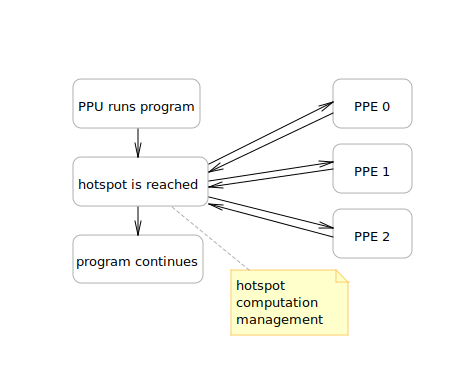
\includegraphics[width=0.7\textwidth]{data/PPUCentricModel}
    \caption[PPE centric configuration]{Program is run on PPE and only hotspots are offloaded to SPEs.
 Offloading means managing SPE context creation and loading as well as managing data transfer and synchronization between PPE and SPEs}
    \label{fg:PPUCentricModel}
\end{figure}

\item SPE server
\par
Another configuration is to have server-like programs running on SPEs that sits and waits offering specific services.
It is very similar to the PPE centric configuration.
Only difference is requirement to the program to be small enough to fit into the SPU local store to avoid the frequent SPE context switching.

\end{enumerate}

\section {Building for the \mbox{Cell/B.E.}}
\par
Actual compilation process is performed using an appropriate tool chain.
The PPE code requires the PPE tool chain and the SPE code requires the SPE one.
But there is a difference between management of the code in linking stage between the PPE and the SPE object files.
It is caused by difference of actual code usage.
While the PPU code resides in the central memory, like in common architectures, the SPU code is loaded into the SPE dynamically and shall be somehow separated from the PPE code.
It is similar to shader programs for graphic accelerators.
They are also loaded into appropriate processors as soon as they are needed so they live separated.

\par
There are two options for SPE code management.
One is to build a shared library and load it explicitly when it shall be used.
Another way is to build a static library and include it into the PPU executable using \mbox{Cell/B.E.} Embedded SPE Object Format (CESOF).
This allows PPE executable objects to contain SPE executable i.e. the SPE binary is embedded within the PPE binary, see figure \ref{fg:SPEEmbedding}.
The SPU program is then referenced as special external structure directly from the PPU code instead of performing shared library loading.
Both ways have advantages and disadvantages which are the same as shared vs. static library usage.
Shared library means better modularity and possibility of code alternation without whole executable rebuilding.
On the other hand additional management of such library is necessary in contrast to a static SPE code into a PPE binary embedding.


\begin{figure}
    \centering
    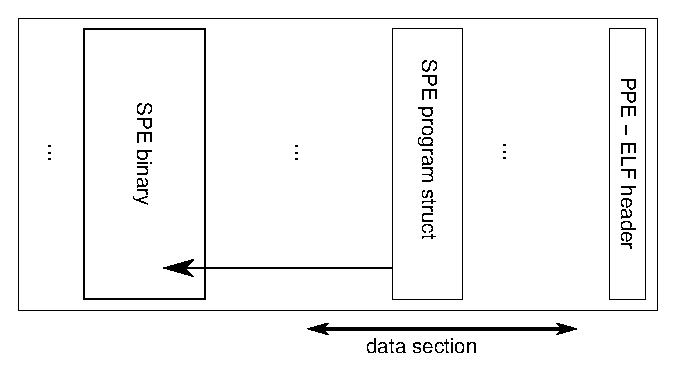
\includegraphics[width=0.8\textwidth]{data/SPEEmbedding}
    \caption[SPE binary embedding]{Illustration how is a SPE binary "embedded" into a PPE binary.
The SPE binary is another section of the PPE binary.
It is reachable through extern struct variable, that contains a pointer to the SPE binary.}
    \label{fg:SPEEmbedding}
\end{figure}



\subsection {Process of application porting for the \mbox{Cell/B.E.}}
\label{sect:portingProcess}

Common process of application porting for the \mbox{Cell/B.E.} processor (figure \ref{fg:appPorting}) consists of next two basic steps:
\begin{enumerate}
\item Hotspots localization
\par
Through profiling of the application on the PPE we find most compute intensive parts, hotspots.
How to profile the application see chapter 5 of \cite{programmersGuide}.\\

\item Hotspot porting for SPE
\par
Each hotspot computation is moved to the SPE i.e. the code adaptation for the SPE features shall be performed.
This means DMA transfers instead of direct memory access, appropriate data structures utilization, etc.
Data movement tuning e.g. different data structures usage can be then performed until satisfactory performance is obtained.

\par
Work distribution among available SPEs shall be performed to accelerate actual computation.
Amount of work performed by particular SPEs should be equal to avoid mutual SPE waiting.
\end{enumerate}

\par
Following additional steps are necessary for application optimization and speed-up.
Performing these steps leads to utilization of all the SPU features such as whole register set utilization, dual-issuing of instructions, SIMD execution and DMA transfers.
More detail in \cite{writingPerfApps}, part 4:

\begin{enumerate}
\item{Multi-buffering}
\par
Data that resides within central memory and are processed by the SPE should be copied into local store before actual computation.
When there are more of the places for the data (buffers) the program can take advantage from asynchronous DMA transfer and can process current buffer while the next data are being transferred into another buffer.
Then the buffers are simply swapped and the SPU need not to wait until the transfer of next data is complete.
See the figure in the paragraph named "Hiding data-access latencies" in \cite{compilerOptions} for illustration.\\

\item{Branch elimination}
\par
Branch less instruction chain is a succession of instructions without any conditional jump.
In other words there is no decision where to continue performed within such succession.
Elimination of branches elongates the branch less instruction chain.
In such a chain all data always go through the same instructions which makes possible to perform SIMDation.
There is variety of branch elimination methods.
Good information resource provides \cite{cellPerformance}.
Branch elimination is probably the most complicated step due to necessity of complete code restructuralization.

\item{SIMDation}
\par
Means rewriting a scalar code into a vectorized one to be able to use SIMD instructions.
In this step the most performance gain could be achieved because of multiple data processing by one instruction.
Every single piece of data should go through the exactly same order of instructions in SIMDized code.
Therefore is necessary to have long branch less instruction chain.
The most important method is arrays of structure to structure of arrays conversion.
The figure in the paragraph called "SIMDizing" in \cite{compilerOptions} shall illustrate the data processing with SIMD instructions.

\par
SIMDizing brings also avoidance of usage a rotation instructions which are necessary to move unaligned data into preferred slot.
Preferred slot is the beginning of a register e.g. for short integer it is the first 16 bits of the register.

\item{Loop unrolling}
\par
Loop body is the code inside curly brackets of the loop.
This code is executed repeatedly until the loop condition is valid.
Loop unrolling means putting more loop bodies serially into the code.
This decrease loop count and elongate the loop body letting the compiler to make more optimizations.
Example:
\begin{verbatim}
for(uint32 i=0; i<32; i++)
{
    printf(".");
}
\end{verbatim}
become (by loop unrolling with factor 2)
\begin{verbatim}
for(uint32 i=0; i<16; i++)
{
    printf(".");
    printf(".");
}
\end{verbatim}
The compiler can do more optimizations e.g. better instruction scheduling and register utilization.

\item{Instruction scheduling}
\par
Proper reorganization of instructions can give more performance in some cases.
This step is performed by the compiler but it is possible to rearrange instructions manually in assembly language.

\item{Branch hinting}
\par
Gives a hint where the program is rather going to continue after future branch to the processor.
It is done through insertion of special instructions.
This step should be again accomplished by the compiler but it is possible to use appropriate assembly language instruction directly within the code.
\end{enumerate}

\begin{figure}
    \centering
    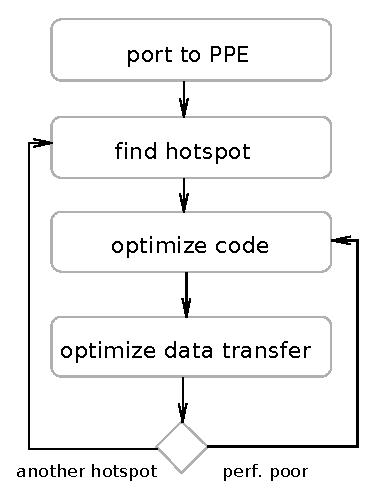
\includegraphics[width=0.5\textwidth]{data/portingCycle}
    \caption[Application porting cycle]{Diagram shows all stages of the process and loops for better performance tuning and other hotspots}
    \label{fg:appPorting}
\end{figure}

\subsection {SPE porting considerations}

\par
The local store size is the main SPE feature that everything spins around while porting a code to the SPE.
On the one hand there are decisions about data transfers.
This means how the data that has to be processed by the SPE will be transferred into local store and vice versa.
How many buffers will be used in case of multi-buffering.
On the other hand is code complexity of the solved problem that influence the size of the final binary.
There is one solution how to use bigger binaries than the local store, SPE overlays.
It is based on division of the binary into segments that are loaded into the SPE on demand in run-time.

\par
Programmer has to take into consideration all these things to make the final binary smaller than the local store.
Everything is big trade-off between the processed data chunk sizes, number of buffers for that chunks and the code lenght.

\par
After the first compilation of a SPU binary from original ported code the final executable will probably exceed the local store size even when the code does not seem as large.
Then a big searching what part of code causes the huge size would begin.
We have gone through several problems with code that is common in non SPE code but cause problems in the SPE code.
Here is the list:
\begin{enumerate}
\item usage of keyword new
\par
There is no memory allocation in the SPE. 
So usage of the \emph{new} keyword is meaningless.
But the SPE compiler accepts it without any complain.

\item usage of std streams
\par
This code:
\begin{verbatim}
#include <iostream>
std::cout << "Hello" << std::endl;
\end{verbatim}
goes through the compiler without complaints but makes the final binary very big.

\par
The reason why the resulting code is too big is probably size of the code within headers that are included when using described features.

\end{enumerate}

\subsection {Speed and compiler options}

\par
There is variety of compiler options.
Usage of them is worth nothing but can increase performance and avoid some kind of bugs.

\par
Mike Acton explains strict aliasing in \cite{strictAliasing}.
One advantage of usage of this feature is positive impact on performance.
Another advantage is fact that it can avoid bugs that would appear as far as in release stage when optimizations flags are used during compilation.
In this stage is really hard to track and debug this kind of bugs.

\par
Another option advises are in \cite{compilerOptions}

\section{Profiling}

\par
Profiling of \mbox{Cell/B.E.} application means rather profiling the SPE part of the application.
There is variety of profiling tools.
The basic one is a dynamic performance analysis which can provide many useful information such as how much time SPE stalled, reasons of the stall, the CPI (cycle per instruction) ratio, branch count, etc.
The next one is a static performance analysis which can illustrate run of a SPE in instruction precision.
These two analysis are evaluated from program run within full system simulator.
Both the methods are well described in tutorial in the cell IDE help which is accessible through menu $\rightarrow$ Help $\rightarrow$ Help Content in the IDE.

\par
Another profiling tools are:
\begin{enumerate}
\item{PDT - performance debugging tool}
\item{OProfile}
\item{CPC - cell performance counter}
\end{enumerate}

These tools collect profiling data that can be further processed with VPA (visual performance analyser), an external tool provided by IBM.
This tool can display the collected data in different charts, time lines or can highlight parts of the code that are worth to improve and many other useful features.
Usage of all these performance tools is described in SDK document "Performance Tools Reference" in \cite{performanceToolRef}.
We wanted to test them all but when we followed the manual instructions we experienced a few obstacles because we worked on PS3.
Lately, we have found out on forums that unfortunately there is poor or none support for these performance tools on PS3.

\chapter{Segmentation}

In this chapter will be segmentation described, listed some techniques. After that level set method will be described along with its relation to segmentation as well as computation issues. //TODO

\subsection{Problem formulation}
Segmentation is process when pixels of input image are split into several subsets (partitions) based on their characteristics or computed properties, such as color, intensity, or texture. Pixels within such partition then have similar features and compose some object in the image.

In more formal way it is a function that assign a segment to pixel:
\begin{equation}
S: S(p) = k
\end{equation}
where p $\in$ pixels of an image and k $\in$ set of segments

Segmentation is used in many domains such as medicine (locating organs, tumors, bones, ...), parsing images from satellite for maps (location buildings, roads, ...), machine vision (fingerprint recognition, face, eyes, or other features recognition). Or such simple tool as well known "magic-stick" tool in popular graphics editing software (Photoshop, GIMP) that performs thresholding segmentation.

Although there were some attempts to find general-purpouse segmentation solution, results were not satisfactory. So there is not yet such general solution. Each domain needs extra approach how to perform the segmentation. Some of them are not even fully automatic so they need assistance of operator (semi-autonomous approaches). In this kind of segmentation, the user (operator) inputs some region and thus give a hint to the algorithm. This is favorite approach in segmentation of structures (organs, etc.) on medical images. An M.D. then plays the role of the operator because of his knowledge of images' content. Some are autonomous but needs some apriory knowledge of some properties of segmentationed object. 

Sometimes segmentation methodes are performed on different resolutions and then combined together. Which means solution from lower resolution is taken as another input (some criterion, etc.) for solution of higher resolution. 

\subsection{Segmentation methodes overview}

Segmentation methodes can be divided into following basic categories:

\begin{enumerate}

  \item Clustering

  These methodes are used do cluster an image into N clusters. They covers the entire image. Two main subsets of methodes are bottom-up and top-bottom. The first one takes each pixel as separeate cluster and then iterate joining these initial clusters (pixels) based on some criterion until there are N cluster in cluster set. The second one pick N (randomly or heuristic based) chosen cluster centers. And then repeats these two step until some convergence condition is met (e.g. no pixels change clusters): assign pixels to clusters based minimalisation of the variance between the pixel and the cluster center and re-compute the cluster centers by averaging all of the pixels in the cluster. 

  \item Histogram-based

  As first, histogram is computed from pixels of the image. Then peaks and valleys in the histogram creates the clusters in the image. Result can be refined by recursively repeated the process. Recursion is stopped when no new more segments appears.

  \item Edge detection

  These methodes segment an image based on its edges. So core of such methodes is some edge-detection algorithm (Canny, Sobel, ...). Discontinuities of found edges that form the segmented object must be overcome some other technique (i.e. based on distance among edges, when two edges are close to each other they are considered to form boundary of segmented object).

  \item Region growing

  This set of methodes are very similar to flood-fill algorithm. It takes a set of seed points and a segmented image. Each seed point is something like pointer to segmented object on the image. Seed points forms initial set of segments. Then iteration through the neighbouring pixels of an segment is performed. In every step of that iteration an neighbour pixel is compared with region - similarity function is calculated. If it is similar enough, the pixel is added to the region.
  Method is highly noise sensitive. The initial seeds can be misplaced due to the noise. So there is another algorithm that is seedless. It starts with a single pixel (region). Its location does not significantly influence final result. Then the iteration over neighbouring pixels are taken just as in seeded growing. If it is different enough (some threshold value is applied), new segment is created.
  Particular approaches differs in definition of the similarity function. While one group uses pixel's properties (intensity, color) directly, another computes some statistical test and the candidate pixel is processed according the test was accepted or rejected.

  \item Graph partitioning

  This approach converts an image into a graph (pixels coresponds the vertices. There is edge between every pair of pixels and edges are weighted with similarity function of the two connected pixels). Then some graph algorithm that cuts off edges and thus partition the graph (image) is then run. Popular algorithms of this category are random walker, minimum mean cut, minimum spanning tree-based algorithm, normalized cut, etc.

  \item Watershed transformation

  The watershed transformation considers the gradient magnitude of an image as a topographic surface. Pixels having the highest gradient magnitude intensities (GMIs) correspond to watershed lines, which represent the region boundaries. Water placed on any pixel enclosed by a common watershed line flows downhill to a common local intensity minimum (LMI). Pixels draining to a common minimum form a catch basin, which represents a segment.

  \item Model based segmentation

  The main idea of this method is to describe segmentationed object statisticaly (construct a probabilistic model) explaining the variation of the shape of the object. In segmention phase is the model used to impose constraints as prior. Searching for such model contains steps like: registration of the training examples to a common pose, probabilistic representation of the variation of the registered samples and statistical corespodence between the model and the image.

  \item  Neural networks segmentation

  Neural Network segmentation relies on processing small areas of an image using a neural network or a set of neural networks. After such processing the decision-making mechanism marks the areas of an image accordingly to the category recognized by the neural network. A type of network designed especially for this, is the Kohonen map.

  \item Level set

Is method that uses matematical implicit model of an segmented object. It is represented as an surface of level set (LS) function defined on volume. Surface is then deformed with forces that are computed from segmented image resulting actual segmentaion of the object.

Whole process can be illustrated in very similar way to flood-filling. Initial surface (e.g. simple circle, for 2D case, as a surface of a distance function from given point) is deformed with forces that has direction of surface normals. When it approaches borders of the object propagation slows down. On borders on the object propagation stops (forces are zero there).

//TODO obrazek

Another illustration uses landscape with a lake. Water is always at constant altitude and the surface of an landscape changes in time. With the changes of the landscape shoreline of the lake changes as well. Landscape represents the LS function and water surface represent the surface i.e. k-level set.

// TODO obrazek

Advantages of the level set method is that it is implicit (no special stuff needed for merging and splitting surfaces), has only few intuitive parameters, can change the topology and can be performed in all dimension without explicit changes in method. 

\end{enumerate}

\subsection{Level set formulation}

Level set method as proposed by Osher and Sethian \cite{sethianLS} provide numerical and matematical mechanisms how to compute surface deformation as time varying iso-values of LS function using partial differential equations (PDE). 
LS function is a signed scalar (distance) function 
\begin{equation}
\psi : U_{x,y,z} \rightarrow R,
\end{equation}
where $U \subset R^3$ is the domain of the volume (note: every definitions will be for 2D case). $\psi$ can be sometimes called embedding. LS is implicit representation of an surface of the segmented object. Surface is then subset of the LS function values
\begin{equation}
\vec{S} = \{\vec{x}\mid \psi(\vec{x}) = k\}
\end{equation}
S is then called an k-isosurface or k-level set of $\psi$. k can be chosen freely, but in most cases it is zero. Surface is then called zero isosurface, zero LS or front in some contexts and corresponds to the actual object contour. 

Surface can be also defined as local mapping $\vec{S}$:
\begin{equation}
\vec{S}: V_r x V_s \rightarrow R^3_{x,y,z},
\end{equation}
where $V x V \subset R^2$. Because of deformation time variable $t \in R^+$ has to be added resulting function S = S(r,s,t). 
Deformation (propagation) of the surface is then described by an evolution equation i.e. differential equation on S. One approach (dynamic) is to use one-parameter family of $\psi$ i.e. $\psi(\vec{x},t)$ changes over time, $\vec{x}$ remains on the k-level set of $\psi$ as it moves and k remains constant. Resulting equation is:
\begin{equation}
\label{deformEq}
\psi(\vec{x}(t),t) = k \Rightarrow \frac{\delta \psi}{\delta t} = - \Delta \psi \centerdot \vec{v}.
\end{equation}
Where v represents movement of point x on deforming surface i.e. positions in time.
All surface movements depend on forces that are based on LS geometry. And LS geometry can be expressed in terms of differential structure of $\psi$. So following version of equation \ref{deformEq} link folmulated:
\begin{equation}
\frac{\delta\psi}{\delta t} = - \Delta \psi \centerdot \vec{v} = - \Delta \psi \centerdot F(\vec{x}, D\psi, D^2\psi, ...),
\end{equation}
where $D^n\psi$ is the set of n-order derivatives of $\psi$ evaluated at x. The term $F(\vec{x}, D\psi, D^2\psi, ...)$ represents some force that influence the movement of a surface point. This equation can applies to every values of k i.e. every LS of function $\psi$ and is basic equation of LS method.

\subsection{Level set computation}

Computation of surface deformation has to be discretized so it is performed on discretized volume i.e. grid. Equation converts the problem to solving nonlinear partial differential equations (PDE). Surface deformation (propagation, movement) is then computed from initial model in cycles representing discrete time steps using this update equation:
\begin{equation}
\psi_{i,j,k}^{n+1} = \psi_{i,j,k}^{n} + \Delta t \Delta \psi_{i,j,k}^{n},
\end{equation}
where the term $\psi_{i,j,k}^{n}$ is discrete aproximation of $\frac{\delta\psi}{\delta t}$ refering to the n-th time step at discrete position i,j,k (which has an counter part in continous domain $\psi(x_i, y_j, z_k)$ ) and $\Delta t \Delta \psi_{i,j,k}^{n}$ is finite forward difference term representing aproximation of the forces influencing the LS (update term). The solution is then succession of steps where new solution is obtained as current solution plus update term.

Discretization of the LS solution brings two problems. Fist one is need of stable and accurate numeric scheme for solving PDE equations. This is solved by proposed 'upwind sheme' by Osher and Sethian. The second one is high computational complexity caused by conversion surface problem into (one dimension higher) volume problem. 
// TODO popsat narocnost
Some 

\subsection{Speed-up approaches}

Because of computational burden of level set solving some speed-up approaches has been proposed. They are usefull only when only single level set is conputed (that is the case of segmentation). In that case us unnecessary compute solution for given timestep over whole domain but only in those parts that are adjacent to the level set (in its neighbourhood). The most known and used are Narrow Bands and Sparse Fields. 

Narrow Bands (proposed by Adalsteinsson and Sethian \cite{sethianFastLS}) computes embedding only within narrow band (tube). Remaining points are set constant to indicate that thay are not in the tube. When LS reach the border of the tube, new tube has to be recalculated based on current LS and new run of embedding computations are performed on this new tube until envolving LS reaches tube borders.

\begin{figure}
    \centering
    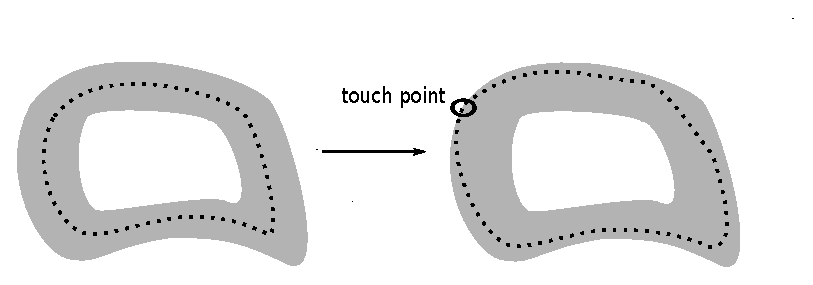
\includegraphics[width=14cm]{data/narrowBands.eps}
    \caption[Narrow bands computation illustration]{Embedding computation is performed only within narrow band (highlighted in grey). When level set touches (highlighted by circle) the border ot the band, new band has to be computed (reinitialized).}
    \label{fg:narrowBands}
\end{figure}

Sparse Fields method (proposed by Whitaker \cite{sparseFilelds}) introduces a scheme in which updates of an embedding are calculated only on the level set. This means that it performs exactly the number of calculations that is needed to calculate next position of the level set. This is the biggest advantage of the method. Points that are adjacent to the level set are called active points (forming active set). Because active points must be adjecant to the LS their positions lie within certain range from the LS. Therefore even values of an embedding in acitive set positions must lie on certain range (active range). When active point value move out from this active range it is no longer the active point and is removed from the active set. And vice versa, the point whose value comes into active range is added into active set. Along the active set there is few layers of points adjecant to the active set organized like peels of an onion. 
Process can be imagined as a tram that lays down tracks before it and picks them up behind.

 Computation of embedding is performed on 

,Several layers around that level set are updated via a distance transform at each iteration.

Even faster method that perform extension and distance reinitialization is $O(N)$ is presented by Peng et al. \cite{pengSparseFields}.

\subsection{Level set segmentation}

The update term from equation //TODO can be further divided into another subterms such as:
\begin{equation}
\psi_{i,j,k}^{n+1} = \psi_{i,j,k}^{n} + \Delta t \Delta \psi_{i,j,k}^{n},
\end{equation}

The most used subterms are propagation (i.e. speed function calculated from segmented image), advection and curvature term (explained later).

Segmentation using LS approach is performed based on a speed function that is calculated from input (segmented image). There are variety speed functions. In this work I use speed function based on threshold $T_{low}$ and $T_{hi}$ of the intensities from the input image. If pixel has intensity value that is within the threshold interval (for maximum speed in the middle of threshold interval), the level set model grows (see figure \ref{fg:speedFunction}). Otherwise it contracts as fast as the pixel has value further from the interval.

\begin{figure}
    \centering
    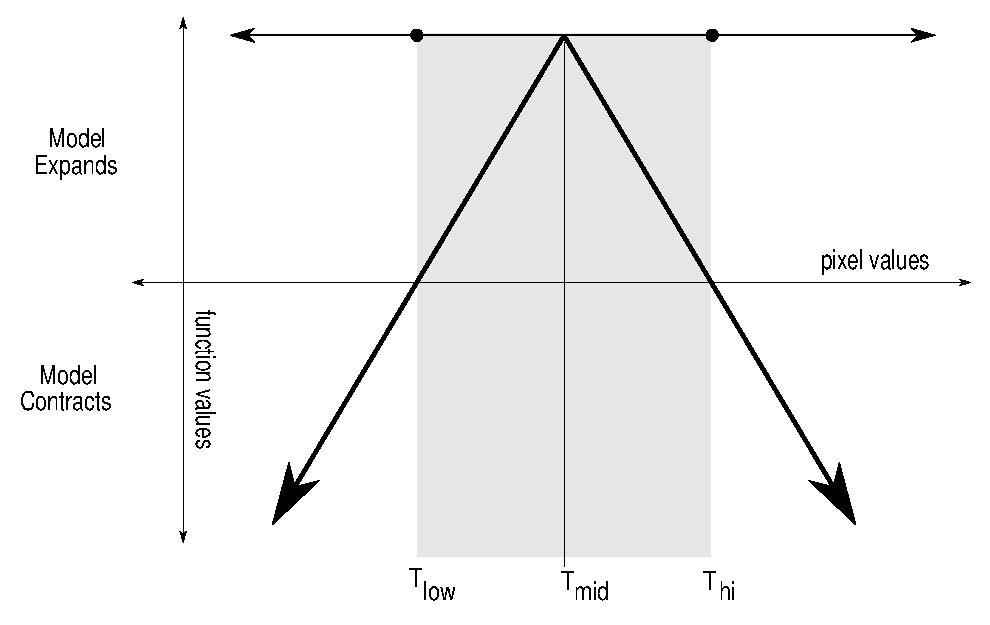
\includegraphics[width=14cm]{data/speedFunction.eps}
    \caption[Graph of thresholding based speed function]{Gray rectangle encloses interval, where is the speed function positive (i.e. the model expands). The fastest expansion is in $T_{mid}$ point that is the middle of that interval}
    \label{fg:speedFunction}
\end{figure}

This is quite natural definition of what we need from the process. Grow as fast as possible where the segmented object lies and contract otherwise.

and such speed functions are
inconsistent with interactive parameter tuning. In general we are concerned with problems
that include a surface curvature term and simultaneously require the model to expand and
contract to match the data.

Tuning of weights of that subterms makes the LS method complex and robust. 

ruzne vzorecky pro diferenci, termy a vahy

segmentace pomoci levelsetu

\section{Level set methodes on streaming devices}

Uvedeni problemu se streamovacimi zarizenimi s odkazem na lefohn_tvcg03.pdf
srovnani jejich moznosti s moznostmi cellu - vyhody nevyhody
\chapter{Results}

In this chapter speed measurements of our application will be presented as well as few pictures of results.
Because we have not speedup the computation over traditional processors discussion of the reasons will follow the results.
We will mention possible changes in design to speed up the execution.
Then some consideration how shall look the algorithm that is well suited for Cell B.E. like.
Chapter will be finished with comparison of complexity of programming for Cell B.E. and conventional processors.

\section{Speed measurements}

\par
Actual speed measurement is performed within \emph{GenerateData} method of the FiniteDifferenceFilter.
Counter is started right after initialization phase (i.e. before main algorithm loop) and stopped right after the loop.
Program memory usage was tuned to use only really necessary amount of memory within measured interval.
Valgrind's massive tool was used for the memory usage tuning.
This was necessary because of the PS3 small memory and because we want to leave swap file untouched during the speed measurement.

\par
Meanwhile this server memory usage tuning some changes was made also within client part.
There was special filter developped.
That filter shrinks data set to given size and cast its voxels to float.
Shrinking is performed by linear interpolation.
The purpose of the float casting is avoiding allocation of additional memory to perform it on the server side.

\par
It is strange that command top shows far bigger memory usage than Valgrind's massif.
We have not care much about it but the idea is that top shows all memory requested from system while massif shows exact memory used by process.

\par
Results of the speed measurement is summarized within Table \ref{tab:runresults}.
Every measurement was run with the same curvature and speed-scaling factors.
But with different initial distance, maximum iterations and seed parameters.
These parameter was set according data set size.

Three different data sets were measured.
All of them was CT images of skull.

\begin{table}
\centering
\begin{tabular}{|c|c|c|c|c|c|c|}
\hline
\multicolumn{7}{|c|}{Measurement results}\\
\hline
data set		&size		&seed		&init.		&max. 		&arch.		&time\\
			&		&		&dist-		&itera-		&		&spend\\
			&		&		&ance		&tions		&		&(sec)\\
\hline
\hline
3slices 		&512x512x3	&[256,256,1]	&40		&800		&Cell B.E.	&16.48\\
(skull 1)		&512x512x3	&[256,256,1]	&40		&800		&i686	.	&1.89\\
\hline
\hline
skull 1			&256x256x80	&[128,110,20]	&20		&500		&Cell B.E.	&471.89\\
			&256x256x80	&[128,110,20]	&20		&500		&i686		&95.23\\
\hline
\hline
skull 1			&256x256x80	&[128,110,20]	&4		&500		&i686		&61.74\\
\hline
\hline
skull 2			&256x256x80	&[128,110,20]	&4		&500		&i686		&55.88\\
\hline
\hline
skull 2			&256x256x80	&[128,128,40]	&4		&500		&i686		&76.9\\
\hline
\end{tabular}
\par
\caption[Measurement results]
{
  Results of speed measurement //TODO
}
\label{tab:runresults}
\end{table}

\section{Pictures}

\section{Reasons of slowdown and possible improvements}

\par
Porting the code to run on SPEs is not sufficient to get more speed from Cell B.E. over traditional processors.
Additional speedup porting phases are necessary.
But our program has another speed pitfalls.

\par
The biggest of them is CellNeighbourhood that represent small segment of an image (the $3^3$ voxel matrix).
It is transferred for every layer (linked chain of nodes) item.
In some parts the both output and status image neighborhoods are transferred.
We wanted to perform the transfer in scatter-gather manner through the DMA lists but we have faced some problems concerning this way of transfer.
The DMA transfers (and specially using DMA lists) are designed for bigger amount of aligned data.
When used for small amounts (smaller that 16bytes per list item) performance goes down because transfer of unaligned data.
When data smaller than 16 bytes (quad-word) are being transferred, every single item is automatically aligned to quad-word address within local store buffer (see Figure \ref{fg:automaticAlignOfSmallData}).

\begin{figure}
    \centering
    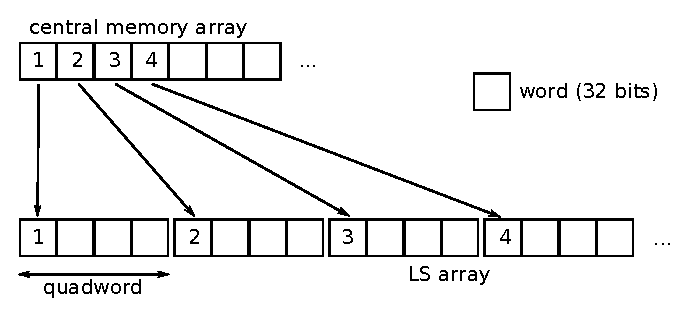
\includegraphics[width=0.8\textwidth]{data/automaticAlignOfSmallData}
    \caption[automatic align of small data]
{
  Illustration of transfer of data that are smaller that quad-word.
  Hardware automatically increase address within local store buffer in such way that every transferred item is quad-word aligned.
}
    \label{fg:automaticAlignOfSmallData}
\end{figure}

This increase required size of buffer that is needed for the transfer.
This can be partially solved by usage of multiple DMA lists (one for each quadword align).
This is illustrated on Figure \ref{fg:multipleDMAList}.
For details see \cite{DMAListIssues}.

\begin{figure}
    \centering
    \includegraphics[width=0.95\textwidth]{data/multipleDMAList}
    \caption[multiple DMA list workaround]
{
  Workaround for transfer in smaller than quad-word chunks.
  Uses more that one DMA list.
  One per quad-word align (e.g. for single bytes 16 DMA lists are needed).
}
    \label{fg:multipleDMAList}
\end{figure}

We have adopted this workaround and used it within the neighborhood transfer.
Because if automatic local store quadword address aligning we had to use a translation table that maps position of actual neigbourhood members into the local store buffer which had to be enlarged appropriately based on data type that stores.
This is working solution but overhead for SPE is incredible and thus useless (see cellNeigbourhood.tcc for details).

\par
\label{neighbourhoodDependecy}
Another problem is order of layer nodes (and thus neighborhoods) processing.
When there are two nodes within one layer that are next to each other and processed subsequently.
Changes made to the first processed neighborhood would not appear to already preloaded next one.
So another merging need to be performed.

\par
This coerced another changes to neighborhood transfer and made the actual transfer unbearably expensive operation.

\par
\label{workDependecy}
Additional pitfall is the situation when sibling nodes are processed by two different SPEs.
Adding nodes to layers is based on information from currently processed node's neighbors.
So it is possible that two different SPE inserts the same nodes more time into one layer because they process sibling nodes (i.e. overlapping neighborhoods).
This makes no changes to output but additional overhead due to processing multiplied nodes.
Solution to this problem would be synchronization among the SPEs.

\par
To speed up the execution improvement of neighbourhood transfers should be done.
This corresponds to data transfer optimization step of porting process (see \ref{fg:appPorting})
In our case this means radical simplification of neighborhood transfers.
This transfers should take only a few instructions to be effective.
Within SDK examples they are performed by simple macros which is probably the most effective way.
In our case simplification if the neighborhood transfer would mean utilization of bigger image parts transport within the DMA transfers to avoid automatic local store alignment for small data transfers.
This would mean a bigger local store array to store the image part but processing of nodes that are associated with the part would be somehow gathered and thus the count of transfers would be less.
Processing of nodes should take into account their spatial information when inserted into a layer and thus to gather the node processing on the bigger neighborhood.
But such computation scheme would coerce complete redesign of application.

\section{Code and design complexity}

\par
Cell B.E. programming means mainly programming for SPEs because of their performance and count.
Because of indirect memory access and need of usage of some multi-bufferring memory transfer scheme the design is quite more complex over common processor.
With another limitation which is the local store size is design of Cell B.E. application a challenge.

\par
Cell B.E. is designed for intensive computation programs.
For programmer this means utilize all SPEs and all their features at maximum level.
It is only possible for certain class of algorithm.
Lets call them streaming parallel algorithm.
But what is it? What is the definition?
Work on our application has showed us what is not the streaming parallel algorithm.
So by negation of features that slow down our program we could get definition of such streaming parallel algorithm:
\begin{enumerate}

\item{Streaming nature}
\par
Data of that program are uniform and can be processed in small pieces (chunks) which are mutually independent which can fit in local store memory.
This means that for one chunk processing is only necessary this chunk and not any part of other chunks.
And when this chunk is once processed is stored and never retrieved for processing again.

\par
For our application this is not true.
At least not for all the input data.
Processing of a sparse field layer (linked chain of nodes) meets the streaming nature.
But processing of parts of underlying images (neighborhoods) associated with this nodes does not.
Neighbourhoods are mutually dependent see \ref{neighbourhoodDependecy}.

\item{Paralel nature}
\par
Input data can be divided into parts which are again mutually independent and which can be sent to particular cores for processing.

\par
For our application is again not true.
Work that is divided among the cores is not independent because of dependency of particular neighborhoods.
See \ref{workDependecy} what causes problems.

\end{enumerate}

\par
When algorithm does not meet the streaming parallel definition then it should not be implemented or changed.
This means e.g. to use different data structures.
In our case, change of the data structure to somehow gather node processing to specific image part would be the change of algorithm we implemented leading to performance gain.
But then this would be the original algorithm any more.

\par
In contrast there are algorithms that fits the streaming paralel algorithm definition.
Among the examples within SDK e.g. thresholding is one of them.
It operates on image that has uniform data - pixels.
It apply simple condition on each pixel which result depends only on the processed pixel.
Processing can be divided into chunks.
These three features meets the streaming condition.
Moreover the data can be divided into independent sets that can be processed by multiple cores (the parallel nature).
Implementation of this algorithm can therefore result huge performance gain on Cell B.E. than conventional processors.

\par
Our work has showed importance of initial consideration and design phase.
When there is more algorithms that are solving desirable problem programmer should think carefully which one will be the best for porting to Cell B.E.
First stage of the initial consideration should be model of the application implementing chosen algorithm.
Thing what kind of data are processed.
If they are uniform.
If they are divisible into chunks.
If the computing can be divided into independent parts i.e. what entity defines amount of work to be done.
These are question that leads to answer if the chosen algorithm is or is not the streaming parallel.
If the answer is no, implementation of that algorithm is rather worthless and will result such suboptimal program as the ours.

\par
Another thing is the code complexity.
Performing the optimisation porting cycle steps utilise leanguage intrinsics for differend kind of special instructions usage of macros for variety of purposes.
These techniques increase actual code complexity whereas may decrease code readability.

\subsection{Algorithm complexity}

\par
There is still another question to be answered.
Is implementation of an algorithm worth at all?
Since only some special products is equipped with Cell B.E. actual data has to be sent to such mashine for computing and results has to ber sent back.
So only complex algorithm where performance gain would be bigger than the time spent in transfer of actual data set are worth to port.
The algorithm we have tried to implement is complex enough to be offloaded to compute on remote machine while the mentioned thresholding would not.
As soon as common machines such as notebooks, desktops are equipped with the Cell B.E. processor even class of such simple image processing algorithms that is implemented in everyday-use software (such as the thresholding or variety of masking, edge detections) could take advantage of the processor.

\chapter{Conclusion}

At the beginning we studied available literature to find out what is actually Cell B.E., what benefits it brings for what price.
What special features it have and what are they good for.
Then we have been trying to install SDK to start actual development process.
During this phase we faced some obstacles like bugs, incompatibilities among tools, libraries that the tools use and even operating system vs. SDK incompatibilities.
So we had to go through variety of forums and other sources to find the solution.
As a side effect we improved our Linux knowledge.
Eventually we managed to install SDK and was able to start developing.
Then we tested variety of libraries, tools and other feature that the SDK brings.
We have chosen sparse field algorithm implementing level set based segmentation to port to Cell B.E. platform.
This is quite complex algorithm to test the platform's potential.
We adopted ITK implementation of that algorithm.
So we had to study ITK toolkit and its internals.
We have also incorporated the whole program into MedV4D framework.
That means we have implemented some new modules that allows using ITK and can offload some part of processing to another machine (that run on Cell B.E.).
Actual porting process started with profiling of existing application.
This step have found out hot spots of the code which can be in turn offloaded to SPE to take advantage of Cell B.E. potential.
But results was quite unexpected so another redesign of application followed.
In this new design almost whole original ITK pipeline was offloaded into SPE.
Big code restructuring was necessary to allow to perform actual computations on SPE.
Finnaly we have able to run the whole algorithm on SPE and thus to measure time need for computations.
The result of measurement showed that simple move the computation to SPE slows down the computations because of insufficient utilization of Cell B.E. features.
We have identified some bottlenecks of the application and discussed possible solutions.
Implementation of these solutions would require whole application redesign using another data structure.
This changes would actually mean change of used algorithm.

\par
We have also discussed differences between programming conventional processors and Cell B.E.
As well as question of actual algorithm complexity and worthiness of porting them to Cell B.E.


\par
The Cell B.E. platform is very interesting for its variations of use scenarios and ability of program tuning and customization.
We think the pallet of tools and features of the Cell B.E. can make it interresting alternative to conventional processors whose lifetime gets shorter due to limitations in manufacturing process.
Cell B.E.'s great potential has already been proven but it is still waiting for wider spectrum of programmers.

\par
If the process of starting developing on Cell B.E. would become simpler we believe much more new programmers would be start.
Nowadays there are plenty of information about Cell B.E. but somehow unsorted or out of date.
The best information source are documents shipped along the SDK.
But they are targeted to contain all the information regardless the level of experience of the reader.
So when a programmer wants to start developing applications on Cell B.E. he would go trough plenty of that information before he can start actual work.
It's a pity there are total lack of information for PS3 users within SDK docs.
This is quite problem when big part of beginners has PS3 available.
There is simply lack of some "cookbook for beginners" with practical information and some howtos.
We believe is such cookbook with some of practical information that potentially may help to some other programmers who would like to start developing for Cell B.E.

\chapter{Tools installation}
As first you have to do is to download actual SDK. Go to http://www-128.ibm.com/developerworks/power/cell/downloads.html?S_TACT=105AGX16&S_CMP=LP. You should download following files:

\begin{enumerate} 
\item SDK 3.1 Installer (cell-install-3.1.0-0.0.noarch.rpm  (11MB))
contains install script and other stuff for SDK installation.
\item SDK 3.1 Developer package ISO image for Fedora 9 (CellSDK-Devel-Fedora_3.1.0.0.0.iso  (434MB))
contains rpm packages that actual SDK is composed from (SDK packages) 
\item SDK 3.1 Extras package ISO image for Fedora 9 (CellSDK-Extras-Fedora_3.1.0.0.0.iso  (34MB))
contains some extra packages for Fedora
\end{enumerate}

Download it wherever you want (even though in documentation is /tmp/cellsdkiso). Lets call the folder, you download it into, ISO_DIR.  First you shall stop the YUM updater daemon.

$$
/etc/init.d/yum-updatesd stop
$$

If this outputs: bash: /etc/init.d/yum-updatesd: No such file or directory, you do not have any YUM updater daemon installed so you can skip this step. Now issue following command to install required utilities for SDK installation

$$
yum install rsync sed tcl wget
$$

Now install the dowloaded installation rpm.

$$
rpm -ivh ISO_DIR/cell-install-3.1.0-0.0.noarch.rpm
$$

After this step you have new stuff in /opt/cell installed. There is SDK installation script (cellsdk) located as well. It is wrapper for YUM that manages the SDK packages. Run it with parameter --help to see the usage. So next step is to run it. 

$$
/opt/cell/cellsdk --iso ISO_DIR -a install
$$

Param --iso tells to use downloaded ISOs and where can be found for mounting them onto loopback device. Param -a disables agreeing licences. Otherwise you have to write some 'yes' to agree. Process begins with setting local YUM repositories pointing to the ISOs. Then all default packages are installed with all their dependecies. To check result of the installation issue

$$
/opt/cell/cellsdk verify
$$

Now we have SDK installed. Lets continue with installation of IDE. It consists again of packages. Now to simplify processing packages install yumex that provides graphical interface to YUM. And lets you simply check packages that you want.

$$
yum install yumex
$$

To install CellIDE run yumex, goto Group View->Development->Cell Development Tools. Check cellide, that is actual IDE (Eclipse with cell concerning stuff) and ibm-java2-i386-jre, that is Java Runtime Environment, JRE needed for running of IDE. And click 'Process Queue'. Note: you should have the ISOs mounted onto loopback devices. Otherwise you get 'Error Downloading Packages' after clicking 'Process Queue'. So you have to mount ISOs whenever you want to install package concerning Cell SDK

$$
/opt/cell/cellsdk --iso ISO_DIR mount
$$

After the installation you have two new folders. /opt/cell/ide that contains the IDE and /opt/ibm/java2-i386-50 where JRE resides. To run the ide you have to specify folder where the JRE is (through -vm param).

$$
/opt/cell/ide/eclipse/eclipse -vm /opt/ibm/java2-i386-50/jre/bin/
$$

The last part of develelopment environment is IBM Full-System Simulator (systemsym). It is not part of ISOs with SDK so you have to download it separately. Visit http://www.alphaworks.ibm.com/tech/cellsystemsim/download and download rpm with the simulator appropriate to the platform you are currently using. Be sure to download fedora 9 version of the simulator (cell-3.1-8.f9.*). Then instal it.

$$
rpm -ivh ISO_DIR/sys
$$

Maybe some dependencies will be missing. So you have to install it. In my case ot was libBLT24 and libtk8.5.

$$
yum install blt tk
$$

Now you have simulator installed. But it has nothing to simulate. Image with image of simulated Fedora 9 system is needed (sysroot image). It is among SDK rpms so install it using yumex (Cell Development Tools -> sysroot\_image).
Now all neccessary stuff is installed. You could start the IDE and start development. But there are some bugs to fix yet. 

If you start IDE and it crashes with unhandled exception it is probably caused by xulrunner library. It is ussually installed with Firefox3. There is following workaround:
\begin{enumerate}
\item download an older version of xulrunner. (e.g. from: http://releases.mozilla.org/pub/mozilla.org/xulrunner/releases/1.8.1.3/contrib/linux-i686/xulrunner-1.8.1.3.en-US.linux-i686-20080128.tar.gz)
\item untar to accessable directory (<XULDIR>)
\item edit the /opt/cell/ide/eclipse/eclipse.ini file as follows:
...
-vmargs
-Dorg.eclipse.swt.browser.XULRunnerPath=<XULDIR>
...
\end{enumerate}
Now you should start the IDE without the crash.

Another issue (stack issue) is with tcl (scripting language that is used for configuration of the systemsym). There is bug with stack size chechking that causes cycling of tcl code. To workeraound this problem you should use ulimit command that changes default environment of linux programs

$$
ulimit -s unlimited
$$

causes that stack is unlimited.

The last is to fix actual tcl script that manages loading the sysroot\_image (21\% issue - loading of the sysroot_image freezes on 21\% so is not started and thats why unusable). It is cause by wrong triggers that are triggerd when some text is output from console by the sysroot_image loading. There is probably triggers that wait for text from previous version of SDK that is never output in the current version. That is why the loading freezes on 21\%. To fix it you have to edit /opt/cell/ide/eclipse/plugins/com.ibm.celldt.simulator.profile.default_3.1.0.200809010950/simulator_init.tcl file. Replace the "Welcome to Fedora Core" string with "Welcome to Fedora" and "INIT: Entering runlevel: 2" with "Starting login process".

It is usefull to create starting script. That solve the stack issue and add systemsim directory to PATH (needed for running).

$$
ulimit -s unlimited
PATH=/opt/ibm/systemsim-cell/bin:$PATH
/opt/cell/ide/eclipse/eclipse -vm /opt/ibm/java2-i386-50/jre/bin
$$

\subsection{Installation of libraries into sysroot\_image}
Because sysroot\_image is provided as image of installed Fedora 9 without CellBE libraries so next step is to install them into sysroot image.

$$
/opt/cell/cellsdk_sync_simulator install
$$

This shell script installs all rpms for ppc and ppc64 platforms that finds in /tmp/cellsdk/rpms. By default these rpms are copied into /tmp/cellsdk/rpms during the install process. If they are not still there (or in installed subdirectory) you have to copy them by hand from ISOs (note: ISOs has to be mounted).

$$
cp /opt/cell/yum-repos/CellSDK-Devel-Fedora/rpms/*.{ppc,ppc64}.rpm /tmp/cellsdk/rpms
$$

\section{Setup CellIDE}

\section{Using examples}

Examples are installed into /opt/cell/sdk/src as tarball. So you have to untar each you want to use. It is good to start with examples and tutorial sources. Each folder has its own makefile that manages makefiles in its subfolders. So you can call only the top level one to build all projects in subfolders or any from the subfolders to build particular projects.

It is convenient to use the sample sources in CellIDE where you can build it as well and create run/debug configuration for running within cell environment. To use the exmaple code (for example /opt/cell/sdk/src/tutorial/simple) create new c++ makefile project. Click right button on it to get into properties. C/C++ general tab -> Paths and Symbols -> Source location. Here you have to add the folder with the sources (/opt/cell/sdk/src/tutorial/simple) by 'create / link folder' button -> advanced -> link to folder in filesystem. Now you have two folders in list. The first one is the original, created during project creation and the other newly linked folder with the source. You can delete the original one since you are not going to use it.
Next is neccassary to set up 'Build directory' to tell the IDE where shall search for makefile. It is C/C++ Build tab. Use 'Workspace' button to specify the folder because it will use workspace_loc variable and thus independent on exact location on filesystem.  

\end{document}